% !TeX root = ..//diffgeo_main.tex

\begin{align}
\ddot{c}^k (t) = - \sum_{ij} \dot{c}^i \dot{c}^j \Gamma^k_{ij}
\end{align}
Wir erhalten also eine gewöhnliche Differentialgleichung zweiter Ordnung.
Diese können wir in zwei Gleichungen erster Ordnung umschreiben.
\begin{align}
&\dot{c}^k (t) = \xi^k(t)\\
&\dot{\xi}^k (t) = - \sum_{ij} \Gamma^k_{ij} \xi^i \xi^j
\end{align}
Auf (Semi-) Riemannschen Mannigfaltigkeiten $(\mfk, g)$ erhalten wir die Geodätische mithilfe des Levi-Civita Zusammenhanges.

\begin{bsp}
\begin{enumerate}
\item $(\R^n, g_{\text{Eukl}})$, $\Gamma^k_{ij}= 0$
\begin{align*}
\ddot{c}^k(t) = 0, \quad \forall t, k\\
\Rightarrow \dot{c}(t) = \text{const.}\\
\Rightarrow c(t) = a t + b
\end{align*}
\item $(\R^n, g_{\text{Minkowski}})$, $\Gamma^k_{ij}= 0$
\begin{align*}
\Rightarrow c(t) = a t + b
\end{align*}
\end{enumerate}
\end{bsp} 

\begin{lem}
\label{lem:geolinear}
Sei $c: I \to \mfk$ eine Geodätische, dann folgt daraus, dass 
\begin{align*}
\tilde{c}(t) = c(\alpha t + \beta), \quad \alpha, \beta \in \R
\end{align*}
ebenfalls eine Geodätische ist.
\end{lem}
\begin{bew}[Beweis Lemma \ref{lem:geolinear}]
\begin{align*}
&\dot{\tilde{c}}^k = \alpha \dot{c}^k (\alpha t + \beta)\\
& \ddot{\tilde{c}}^k = \alpha^2 \ddot{c}^k (\alpha t + \beta)
\end{align*}
\end{bew}
\begin{defs}[Parametrisierung nach der Bogenlänge]
Sei $(\mfk, g)$ eine (Semi-) Riemannsche Mannigfaltigkeit.
Eine Kurve $c: I \to \mfk$ ist
\begin{itemize}
\item parametrisiert nach der Bogenlänge, falls
\begin{align}
g(\dot{c}, \dot{c}) = 1
\end{align}
\item proportional zu Bogenlänge parametrisiert, falls
\begin{align}
g(\dot{c}, \dot{c}) = \alpha > 0, \quad \alpha \ \mathrm{const.}
\end{align}
\end{itemize}
\end{defs}
\textbf{Übung:} Geodätische sind immer proportional zur Bogenlänge parametrisiert.\\

Wir brauchen lokale Existenz und Eindeutigkeit für unsere Lösungen.\\
\textbf{Erinnerung:} Sei $O \in J \subset \R$ ein Intervall und
\begin{align*}
\left. \begin{array}{l}
U \subset \R^m\\
V \subset \R^n
\end{array}
\right\} 
\mathrm{offen}
\end{align*}
und $f: J \times U \times V \to \R^n$ glatt.
Dann existiert für jedes $(u, v) \in U \times V$ ein eindeutiges maximales Intervall $I_{u, v} \subset J$, sodass eine eindeutige Funktion
$x_{u,v}: I_{u, v} \to V$ existiert mit:
\begin{align*}
&\dot{x}_{u, v} (t) = f(t, u, x_{u,v}(t))\\
&x_{u, v}(0) = v
\end{align*}
Ferner ist 
\begin{align*}
O = \{ (t, u, v) \in J \times U \times V  \vert t \in I_{u, v}\}
\end{align*}
offen und
\begin{align*}
(t, u, v) \mapsto x_{u,v}(t)
\end{align*}
ist glatt.\\
\textbf{Literaturhinweis:} \textit{Fundamentals of differential geometry} Kapitel 4
\begin{satz}
Sei $\mfk$ ein Mannigfaltigkeit mit dem Zusammenhang $\nabla$.
\begin{enumerate}
\item \textbf{(Existenz)} Zu jedem $p \in \mfk$, $v \in T_p \mfk$ existiert ein $I$ und eine Geodätische
\begin{align*}
c: I \to \mfk ,
\end{align*}
mit $0\in I$, $c(0) = p$ und $\dot{c}(0)=v$
\item \textbf{(Eindeutigkeit)} Sind $c_1$, $c_2 : I_i \to \mfk$ Geodätische mit $c_1(0) = c_2(0)$ und $\dot{c}_1 (0) = \dot{c}_2 (0)$, dann folgt:
\begin{align*}
c_1(t) = c_2(t), \quad \forall t \in I_1 \cup I_2
\end{align*}
\item Gegeben $p, v$ dann existiert ein eindeutiges maximal offenes Intervall $I_v \ni 0$ und maximale Geodätische (Also Geodätische auf dem maximalen Intervall)
\begin{align*}
c_v : I_v \to \mfk ,
\end{align*}
mit $\dot{c}_v (0) = v$ und $c(0)= \pi (v)$
\item Die Menge
\begin{align*}
O = \{ (t, v) \in \R \times T \mfk \ \vert \ t \in I_v \}
\end{align*}
ist offen und 
\begin{align*}
&c: O \to \mfk\\
& (t,v) \mapsto c_v(t)
\end{align*}
sst glatt.
\end{enumerate}
\end{satz}
\begin{defs}[Vollständigkeit]
Ein Zusammenhang auf $\mfk$ heißt vollständig, falls $O = \R \times T\mfk$.
Das heißt alle Geodätischen sind auf ganz $\R$ definiert.\\
Eine (Semi-) Riemannsche Mannigfaltigkeit heißt vollständig falls der Levi-Civita Zusammenhang vollständig ist.
\end{defs}
\begin{bem}
Ist $f: \mfk \to \mfka$ eine Geodätische, dann folgt daraus, dass $f\circ c: I \to \mfka$ eine Geodätische ist
\end{bem}
\begin{bew}
Übung (Hinweis: Isometrien erhalten Christoffel Symbole).
\end{bew}
Sei $\varphi : \mfk \to \mfk$ ein Diffeomorphismus.
Die Menge der Fixpunkte von $\varphi$ ist:
\begin{align}
\fix (\varphi) = \{ p \in \mfk \vert \varphi (p) = p\} 
\end{align}
\begin{satz}
\label{satz:fixpunkte}
Sei $(\mfk, g)$ ein (Semi-) Riemannsche Mannigfaltigkeit  und $\varphi \in \isom (\mfk, g)$.
Sei $p \in \fix (\varphi)$ und $v \in T_p \mfk$ mit $\dd \varphi_p (v) = v$.
Dann hat die Geodätische
\begin{align}
c_v : I_v \to \mfk ,
\end{align}
die Eigenschaft: $c_v(t) \in \fix (\varphi)$ für alle $t \in I_v$
\end{satz}
\begin{bew}[Beweis Satz \ref{satz:fixpunkte}]
$\varphi \circ c_v (t) = \tilde{c}(t)$ ist eine Geodätische mit
\begin{align*}
&\tilde{c}(0) = \varphi (p) = p\\
&\dot{\tilde{c}}(0) = \dd \varphi (v) = v\\
&\Rightarrow \tilde{c}(t) = v(t), \quad \forall t \in I\\
&\Rightarrow \varphi (c_v(t)) = c_v (t)\\
&\Rightarrow c_v (t) \in \fix (\varphi)
\end{align*}
\end{bew}

\begin{bsp}[Geodätische auf $S^n$]
\begin{align}
S^n = \{ x \in \R^{n+1} \vert \langle x, x\rangle  = 1\} \subset (\R^{n+1}, \langle \cdot, \cdot \rangle_{\mathrm{Eukl}})
\end{align}
Hier ist $T_p S^n = p^\perp$.
Dies wird in Abbildung \ref{img:sphere_tangent_space} veranschaulicht.
\begin{figure}[H]
\centering
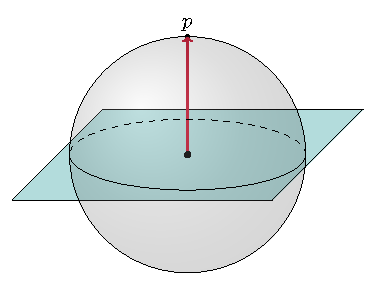
\includegraphics[width=0.4\linewidth]{figures/tikz/sphere_tangent_space.pdf}
\caption{Veranschaulichung des Tangentialraumes des $S^n$ am Punkt $p$}
\label{img:sphere_tangent_space}
\end{figure} 	
Für $u, v \in p^\perp$ gilt:
\begin{align*}
& \langle v, p \rangle = 0\\
& \langle p, v \rangle = 0\\
& \langle p, p \rangle = 1
\end{align*}
Wir haben die Standardmetrik mit:
\begin{align*}
g_p (v, w) = \langle v, w\rangle .
\end{align*}
Sei $A \in O(n+1)$
\begin{align*}
& A: \R^{n+1} \to \R^{n+1}\\
& v \mapsto A v
\end{align*}
Für die Metrik $g$ gilt:
\begin{align*}
g_p (v, w) &= \langle v, w\rangle\\
&= \langle Av, Aw \rangle\\ 
&= g_{A_p} (A_v, A_w)\\
\Rightarrow A \subset \isom (S^n)
\end{align*}
Seien $p \in S^n$ und $v \in T_p S^n = p^\perp$.
$E = \mathrm{span} \{ v, p \} \subset \R^n$ ist eine Ebene.
Sei $A_E : \R^{n+1} \to \R^{n+1}$ die Speigelung an $E$.
Betrachte den Vektor $(p, v, \underbrace{e_3, \dots, e_{n+1}}_{E^\perp})$
\begin{align*}
&A_E (p) = p\\
& A_E (v) = v\\
& A_E(e_i) = - e_i, \quad \forall i
\end{align*}
$A_E \in O(n+1)  \subset \isom (S^n)$.
$\fix (A) = E \cup S^n$ ist ein Kreis.
\begin{align}
&c_v : I_v S^n\\
&c_v(t) = \cos (\alpha t) p + \sin (\alpha t) \frac{v}{\norm{v}}
\end{align}
\begin{figure}[H]
\centering
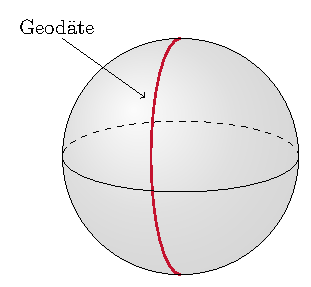
\includegraphics[width=0.4\linewidth]{figures/tikz/geodesic_sphere.pdf}
\caption{Geodäte auf $S^n$}
\label{img:sphere_tangent_space}
\end{figure} 	
Mit der Anfangsbedingung $\dot{c}_v (0) = v$ folgt $\alpha = \norm{v}$.\\
Es folgt, dass $S^n$ vollständig ist, da $I_v = \R$.
\end{bsp}
\textbf{Übung:} Finde Geodätische für den Hyperbolischen Raum $H^n$.
